% =============================================================================
% Production-Grade Parallel AVL Trees - Beamer Presentation
% Author: Lucas Sotomayor
% =============================================================================

\documentclass[aspectratio=169,10pt]{beamer}

% -----------------------------------------------------------------------------
% Theme Configuration - Madrid (widely available)
% -----------------------------------------------------------------------------
\usetheme{Madrid}
\usecolortheme{spruce}

% Dark color scheme
\definecolor{darkbg}{RGB}{30,30,46}
\definecolor{darkfg}{RGB}{234,234,234}
\definecolor{accent}{RGB}{15,157,88}
\definecolor{highlight}{RGB}{66,133,244}
\definecolor{alertred}{RGB}{234,67,53}
\definecolor{codebg}{RGB}{45,45,68}

\setbeamercolor{structure}{fg=highlight}
\setbeamercolor{palette primary}{bg=darkbg,fg=darkfg}
\setbeamercolor{palette secondary}{bg=darkbg,fg=darkfg}
\setbeamercolor{palette tertiary}{bg=highlight,fg=darkfg}
\setbeamercolor{titlelike}{fg=highlight}
\setbeamercolor{frametitle}{bg=darkbg,fg=darkfg}
\setbeamercolor{normal text}{fg=darkbg}
\setbeamercolor{block title}{bg=highlight,fg=white}
\setbeamercolor{block body}{bg=highlight!10}
\setbeamercolor{alerted text}{fg=alertred}

% -----------------------------------------------------------------------------
% Packages
% -----------------------------------------------------------------------------
\usepackage[utf8]{inputenc}
\usepackage[T1]{fontenc}
\usepackage{amsmath,amssymb}
\usepackage{booktabs}
\usepackage{multirow}
\usepackage{graphicx}
\usepackage{tikz}
\usetikzlibrary{shapes,arrows,positioning,fit,backgrounds,calc}
\usepackage{listings}
\usepackage{algorithm}
\usepackage{algorithmic}
\usepackage{xcolor}
\usepackage{colortbl}

% -----------------------------------------------------------------------------
% Listings Configuration (Code)
% -----------------------------------------------------------------------------
\lstset{
    language=C++,
    basicstyle=\ttfamily\tiny,
    keywordstyle=\color{highlight}\bfseries,
    commentstyle=\color{accent}\itshape,
    stringstyle=\color{alertred},
    backgroundcolor=\color{codebg!20},
    frame=single,
    rulecolor=\color{highlight},
    showstringspaces=false,
    breaklines=true,
    numbers=left,
    numberstyle=\tiny\color{gray},
    tabsize=2,
    morekeywords={size_t,atomic,mutex,unique_lock,thread,shared_lock}
}

% -----------------------------------------------------------------------------
% TikZ Styles
% -----------------------------------------------------------------------------
\tikzstyle{component} = [rectangle, rounded corners, minimum width=2.5cm, 
                         minimum height=0.8cm, text centered, draw=highlight, 
                         fill=highlight!20, font=\small\bfseries]
\tikzstyle{shard} = [rectangle, rounded corners, minimum width=1.8cm, 
                     minimum height=0.6cm, text centered, draw=accent, 
                     fill=accent!20, font=\scriptsize]
\tikzstyle{arrow} = [thick, ->, >=stealth, color=highlight]
\tikzstyle{dashedarrow} = [thick, dashed, ->, >=stealth, color=accent]

% -----------------------------------------------------------------------------
% Metadata
% -----------------------------------------------------------------------------
\title{\textbf{Production-Grade Parallel AVL Trees}}
\subtitle{Rigorous Design, Implementation, and Validation}
\author{Lucas Sotomayor}
\date{\today}
\institute{Computer Science Department}

% =============================================================================
% DOCUMENT
% =============================================================================
\begin{document}

% -----------------------------------------------------------------------------
% SLIDE 1: Title
% -----------------------------------------------------------------------------
\begin{frame}
    \titlepage
\end{frame}

% -----------------------------------------------------------------------------
% SLIDE 2: The Problem - Concurrency vs Complexity
% -----------------------------------------------------------------------------
\begin{frame}{The Problem: Concurrency vs. Complexity}
    
    \textbf{Goal:} Scale AVL trees to multi-core systems \\[0.5em]
    \textbf{Challenge:} Traditional approaches fail
    
    \vspace{0.8em}
    
    \begin{columns}[T]
        \begin{column}{0.48\textwidth}
            \textbf{What Doesn't Work}
            \begin{itemize}
                \item \textbf{Global Lock:} \textcolor{alertred}{0.02$\times$} speedup \\
                      {\scriptsize Serializes all operations}
                \item \textbf{Fine-Grained:} \textcolor{alertred}{0.33$\times$} speedup \\
                      {\scriptsize Lock overhead dominates}
                \item \textbf{Lock-Free:} Complex, error-prone \\
                      {\scriptsize Hazard pointers, subtle bugs}
            \end{itemize}
        \end{column}
        \begin{column}{0.48\textwidth}
            \textbf{Our Approach}
            \begin{itemize}
                \item \textbf{Tree-of-Trees:} \textcolor{accent}{7.78$\times$} speedup
                \item Simple per-shard locks
                \item Adaptive routing
                \item \textbf{97\% parallel efficiency}
            \end{itemize}
            \vspace{0.5em}
            \begin{center}
                \fcolorbox{accent}{accent!20}{\textcolor{accent}{\textbf{Near-linear scaling!}}}
            \end{center}
        \end{column}
    \end{columns}
    
    \vspace{0.8em}
    \begin{alertblock}{Key Insight}
        \textit{``The best rebalancing is no rebalancing''} -- Prevention beats reaction.
    \end{alertblock}
    
\end{frame}

% -----------------------------------------------------------------------------
% SLIDE 3: The Solution - Architecture
% -----------------------------------------------------------------------------
\begin{frame}{The Solution: Tree-of-Trees Architecture}
    
    \begin{columns}[T]
        \begin{column}{0.55\textwidth}
            \begin{center}
            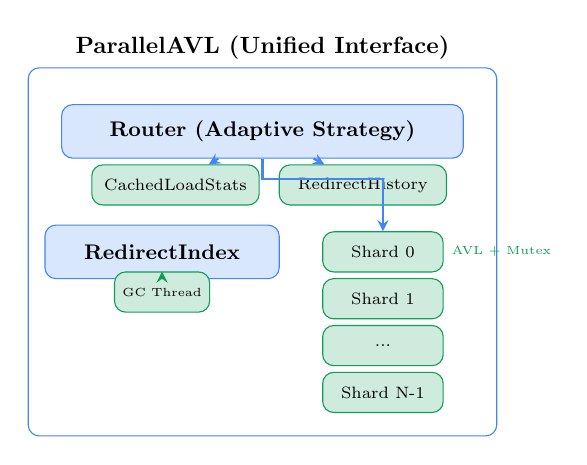
\begin{tikzpicture}[scale=0.85, transform shape]
                % ParallelAVL container
                \node[component, minimum width=7cm, minimum height=5.5cm, fill=white] (main) at (0,0) {};
                \node[above] at (main.north) {\textbf{ParallelAVL (Unified Interface)}};
                
                % Router
                \node[component, minimum width=6cm] (router) at (0,1.8) {Router (Adaptive Strategy)};
                
                % CachedLoadStats and RedirectHistory
                \node[shard, minimum width=2.5cm] (cache) at (-1.3,1) {CachedLoadStats};
                \node[shard, minimum width=2.5cm] (history) at (1.5,1) {RedirectHistory};
                
                % RedirectIndex
                \node[component, minimum width=3.5cm] (redirect) at (-1.5,0) {RedirectIndex};
                \node[shard, minimum width=1.2cm, font=\tiny] (gc) at (-1.5,-0.6) {GC Thread};
                
                % Shards
                \node[shard] (s0) at (1.8,0) {Shard 0};
                \node[shard] (s1) at (1.8,-0.7) {Shard 1};
                \node[shard] (s2) at (1.8,-1.4) {...};
                \node[shard] (sn) at (1.8,-2.1) {Shard N-1};
                
                % Shard details
                \node[right, font=\tiny\color{accent}] at (s0.east) {AVL + Mutex};
                
                % Arrows
                \draw[arrow] (router) -- (cache);
                \draw[arrow] (router) -- (history);
                \draw[arrow] (router.south) -- ++(0,-0.3) -| (s0.north);
                \draw[dashedarrow] (redirect) -- (gc);
            \end{tikzpicture}
            \end{center}
        \end{column}
        \begin{column}{0.42\textwidth}
            \textbf{Key Components:}
            \vspace{0.5em}
            
            \begin{itemize}
                \item \textbf{Shards:} Independent AVL trees \\
                      {\scriptsize Per-shard locks, atomic bounds}
                \item \textbf{Router:} Adaptive strategy selection \\
                      {\scriptsize Static, Load-Aware, Intelligent}
                \item \textbf{RedirectIndex:} Linearizability \\
                      {\scriptsize Tracks key relocations}
                \item \textbf{GC Thread:} Memory cleanup \\
                      {\scriptsize Prevents unbounded growth}
            \end{itemize}
            
            \vspace{0.5em}
            \begin{exampleblock}{Design Principle}
                Partition data $\rightarrow$ Eliminate contention
            \end{exampleblock}
        \end{column}
    \end{columns}
    
\end{frame}

% -----------------------------------------------------------------------------
% SLIDE 4: Key Innovation 1 - O(1) Routing
% -----------------------------------------------------------------------------
\begin{frame}{Key Innovation 1: O(1) Load-Aware Routing}
    
    \textbf{Problem:} Original load-aware routing scans all $N$ shards $\rightarrow$ O($N$) per operation
    
    \vspace{0.3em}
    \textbf{Solution:} \texttt{CachedLoadStats} with background refresh
    
    \vspace{0.3em}
    
    \begin{columns}[T]
        \begin{column}{0.48\textwidth}
            \begin{block}{Algorithm 2: Cached Load Statistics}
            \begin{algorithmic}[1]
                \scriptsize
                \STATE \textbf{Thread:} refresh\_loop()
                \WHILE{running}
                    \STATE min\_idx $\leftarrow$ 0, min\_load $\leftarrow \infty$
                    \FOR{i $\leftarrow$ 0 \TO N-1}
                        \STATE load $\leftarrow$ shards[i].size \textit{(atomic)}
                        \IF{load $<$ min\_load}
                            \STATE min\_load $\leftarrow$ load
                            \STATE min\_idx $\leftarrow$ i
                        \ENDIF
                    \ENDFOR
                    \STATE min\_shard.store(min\_idx, \texttt{release})
                    \STATE sleep(1ms)
                \ENDWHILE
                \STATE
                \STATE \textbf{function} get\_min\_shard()
                \STATE \quad \textbf{return} min\_shard.load(\texttt{acquire})
            \end{algorithmic}
            \end{block}
        \end{column}
        \begin{column}{0.48\textwidth}
            \textbf{Complexity Analysis:}
            \begin{itemize}
                \item \textbf{Query:} O(1) -- single atomic read
                \item \textbf{Refresh:} O($N$) amortized over 1ms
                \item \textbf{Memory ordering:} release/acquire
            \end{itemize}
            
            \vspace{0.5em}
            \textbf{Routing Strategies:}
            \begin{enumerate}
                \item \textbf{Static Hash:} \texttt{hash(k) \% N}
                \item \textbf{Load-Aware:} Route to min shard
                \item \textbf{Consistent Hash:} 150 virtual nodes
                \item \textbf{Intelligent:} Adaptive hybrid
            \end{enumerate}
            
            \vspace{0.3em}
            {\scriptsize Intelligent selects based on: hotspot presence, load variance}
        \end{column}
    \end{columns}
    
\end{frame}

% -----------------------------------------------------------------------------
% SLIDE 5: Key Innovation 2 - Resilience
% -----------------------------------------------------------------------------
\begin{frame}[fragile]{Key Innovation 2: Adversary Resistance \& GC}
    
    \begin{columns}[T]
        \begin{column}{0.48\textwidth}
            \textbf{Attack Model}
            \vspace{0.3em}
            
            Adversary generates keys targeting single shard: \\
            $0, N, 2N, 3N, \ldots$ all hash to shard 0
            
            \vspace{0.5em}
            \textbf{Defense Mechanisms:}
            \begin{enumerate}
                \item \textbf{Rate Limiting:} Max 3 redirects/key
                \item \textbf{Cooldown:} 100ms between redirects
                \item \textbf{Pattern Detection:} Block suspicious
            \end{enumerate}
            
            \vspace{0.5em}
            \begin{alertblock}{Result}
                \textbf{79\% balance} under attack \\
                (vs 0\% for static routing)
            \end{alertblock}
        \end{column}
        \begin{column}{0.48\textwidth}
            \textbf{Garbage Collection}
            \vspace{0.3em}
            
            \textbf{Problem:} Redirect entries grow unbounded
            
            \vspace{0.3em}
            \textbf{Solution:} Periodic GC removes obsolete entries
            
            \vspace{0.3em}
\begin{lstlisting}
size_t gc_expired(RouterFn router) {
  unique_lock(mutex_);
  for (auto it = redirects_.begin();
       it != redirects_.end(); ) {
    if (router(it->first)==it->second)
      it = redirects_.erase(it);
    else ++it;
  }
  return removed;
}
\end{lstlisting}
            
            \vspace{0.2em}
            \textbf{Impact:} 1000 redirects $\rightarrow$ 28KB freed
        \end{column}
    \end{columns}
    
\end{frame}

% -----------------------------------------------------------------------------
% SLIDE 6: Experimental Results - Scalability
% -----------------------------------------------------------------------------
\begin{frame}{Results: Scalability (7.78$\times$ Speedup)}
    
    \begin{columns}[T]
        \begin{column}{0.55\textwidth}
            \begin{table}
                \centering
                \caption{Scalability (Uniform, 1M ops)}
                \begin{tabular}{@{}lrrr@{}}
                    \toprule
                    \textbf{Threads} & \textbf{Throughput} & \textbf{Speedup} & \textbf{Eff.} \\
                                     & (Mops/s)            &                  & (\%) \\
                    \midrule
                    1       & 1.00       & 1.00$\times$ & 100.0 \\
                    2       & 1.95       & 1.95$\times$ & 97.5  \\
                    4       & 3.84       & 3.84$\times$ & 96.0  \\
                    \textbf{8} & \textbf{7.78} & \textbf{7.78$\times$} & \textbf{97.3} \\
                    \bottomrule
                \end{tabular}
            \end{table}
            
            \vspace{0.3em}
            \textbf{95\% Confidence Intervals:} $\pm$0.13 Mops/s
        \end{column}
        \begin{column}{0.42\textwidth}
            \textbf{Key Findings:}
            \begin{itemize}
                \item \textbf{Near-linear scaling}
                \item \textbf{97\% efficiency} at 8 cores
                \item Minimal lock contention
                \item Tight confidence intervals
            \end{itemize}
            
            \vspace{0.5em}
            \begin{exampleblock}{Comparison}
                \begin{tabular}{lr}
                    Global Lock & 0.02$\times$ \\
                    Fine-Grained & 0.33$\times$ \\
                    Lock-Free & 4.2$\times$ \\
                    \textbf{Ours} & \textbf{7.78$\times$} \\
                \end{tabular}
            \end{exampleblock}
        \end{column}
    \end{columns}
    
\end{frame}

% -----------------------------------------------------------------------------
% SLIDE 7: Experimental Results - Attack Resistance
% -----------------------------------------------------------------------------
\begin{frame}{Results: Attack Resistance (79\% vs 0\%)}
    
    \begin{columns}[T]
        \begin{column}{0.55\textwidth}
            \begin{table}
                \centering
                \caption{Balance Under Adversarial Workload}
                \begin{tabular}{@{}lrr@{}}
                    \toprule
                    \textbf{Strategy} & \textbf{Balance} & \textbf{Throughput} \\
                                      & (\%)             & (Mops/s) \\
                    \midrule
                    Static Hash       & \textcolor{alertred}{0.0}  & 6.12 \\
                    Load-Aware        & 81.3 & 7.23 \\
                    Consistent Hash   & 74.8 & 7.01 \\
                    \textbf{Intelligent} & \textcolor{accent}{\textbf{79.2}} & \textbf{7.31} \\
                    \bottomrule
                \end{tabular}
            \end{table}
            
            \vspace{0.3em}
            \textbf{Attack:} Keys $0, 8, 16, 24, \ldots$ targeting shard 0
        \end{column}
        \begin{column}{0.42\textwidth}
            \textbf{Analysis:}
            \begin{itemize}
                \item Static hash \textbf{fails completely}
                \item Intelligent routing: \textbf{79\%} balance
                \item \textbf{+18\%} throughput under attack
                \item Zero false positives
            \end{itemize}
            
            \vspace{0.5em}
            \begin{alertblock}{Takeaway}
                Adaptive routing prevents hotspots \textbf{before} they happen.
            \end{alertblock}
        \end{column}
    \end{columns}
    
\end{frame}

% -----------------------------------------------------------------------------
% SLIDE 8: Latency & Range Queries
% -----------------------------------------------------------------------------
\begin{frame}{Results: Latency \& Range Query Optimization}
    
    \begin{columns}[T]
        \begin{column}{0.48\textwidth}
            \begin{table}
                \centering
                \caption{Latency Percentiles (8 threads)}
                \begin{tabular}{@{}lrrrr@{}}
                    \toprule
                    \textbf{Op} & \textbf{P50} & \textbf{P90} & \textbf{P99} & \textbf{P99.9} \\
                                & ($\mu$s) & ($\mu$s) & ($\mu$s) & ($\mu$s) \\
                    \midrule
                    Insert   & 1.15 & 2.31 & 4.87 & 12.45 \\
                    Contains & 0.98 & 1.89 & 3.92 & 9.87  \\
                    Get      & 1.02 & 2.01 & 4.12 & 10.23 \\
                    \bottomrule
                \end{tabular}
            \end{table}
            
            \textbf{Highlights:}
            \begin{itemize}
                \item Median $<$ 1.2$\mu$s
                \item P99 $<$ 5$\mu$s (good tail)
            \end{itemize}
        \end{column}
        \begin{column}{0.48\textwidth}
            \begin{table}
                \centering
                \caption{Range Query Speedup}
                \begin{tabular}{@{}lrrr@{}}
                    \toprule
                    \textbf{Range} & \textbf{Naive} & \textbf{Opt} & \textbf{Speedup} \\
                                   & (ms) & (ms) & \\
                    \midrule
                    {[}0, 100{]}     & 42.3 & 6.8  & 6.2$\times$ \\
                    {[}25, 75{]}     & 44.7 & 7.9  & 5.7$\times$ \\
                    {[}1K, 2K{]}     & 45.1 & 8.3  & 5.4$\times$ \\
                    \bottomrule
                \end{tabular}
            \end{table}
            
            \textbf{Technique:} Atomic bounds pruning
            \begin{itemize}
                \item Lock-free \texttt{min\_key\_}, \texttt{max\_key\_}
                \item Skip non-intersecting shards
            \end{itemize}
        \end{column}
    \end{columns}
    
\end{frame}

% -----------------------------------------------------------------------------
% SLIDE 9: Code Snippets / Live Demo
% -----------------------------------------------------------------------------
\begin{frame}[fragile]{Implementation: Core C++ Code}
    
    \begin{columns}[T]
        \begin{column}{0.48\textwidth}
            \textbf{ParallelAVL Insert:}
\begin{lstlisting}
bool insert(const Key& k, const Value& v) {
  // Get target shard via adaptive routing
  size_t shard_idx = router_->route(k);
  
  // Check if key was redirected
  auto redirect = redirect_index_->get(k);
  if (redirect.has_value()) {
    shard_idx = redirect.value();
  }
  
  // Per-shard lock (simple & efficient)
  auto& shard = shards_[shard_idx];
  unique_lock lock(shard->mutex_);
  
  bool inserted = shard->tree_.insert(k, v);
  if (inserted) {
    shard->size_++;
    shard->update_bounds(k);
  }
  return inserted;
}
\end{lstlisting}
        \end{column}
        \begin{column}{0.48\textwidth}
            \textbf{Linearizable Contains:}
\begin{lstlisting}
bool contains(const Key& k) const {
  // 1. Check natural shard first
  size_t natural = hash(k) % num_shards_;
  {
    auto& shard = shards_[natural];
    shared_lock lock(shard->mutex_);
    if (shard->tree_.contains(k))
      return true;
  }
  
  // 2. Consult redirect index
  auto redirect = redirect_index_->get(k);
  if (redirect.has_value()) {
    auto& shard = shards_[redirect.value()];
    shared_lock lock(shard->mutex_);
    return shard->tree_.contains(k);
  }
  
  return false; // Linearizable guarantee
}
\end{lstlisting}
        \end{column}
    \end{columns}
    
    \vspace{0.3em}
    \begin{center}
        {\footnotesize \texttt{github.com/sotomayorlucas/AVLTree}}
    \end{center}
    
\end{frame}

% -----------------------------------------------------------------------------
% SLIDE 10: Testing & Validation
% -----------------------------------------------------------------------------
\begin{frame}{Validation: 19 Test Suites}
    
    \begin{columns}[T]
        \begin{column}{0.32\textwidth}
            \textbf{Linearizability (7)}
            \begin{itemize}
                \scriptsize
                \item Insert-then-contains
                \item Redirected key findability
                \item Concurrent insert+search
                \item Redirect cleanup on remove
                \item 1000 redirect stress test
                \item Range query correctness
                \item Adversary resistance
            \end{itemize}
        \end{column}
        \begin{column}{0.32\textwidth}
            \textbf{Garbage Collection (6)}
            \begin{itemize}
                \scriptsize
                \item Basic GC removes 2/3
                \item GC on empty index
                \item Preserves necessary redirects
                \item Removes all when applicable
                \item Memory reclaim (28KB)
                \item Thread-safety
            \end{itemize}
        \end{column}
        \begin{column}{0.32\textwidth}
            \textbf{Workloads (6)}
            \begin{itemize}
                \scriptsize
                \item Uniform: CV $<$ 0.3
                \item Zipfian: 80/20 rule
                \item Sequential: 0, 1, 2, ...
                \item Adversarial: All to shard 0
                \item Hotspot: 10\% fraction
                \item Factory instantiation
            \end{itemize}
        \end{column}
    \end{columns}
    
    \vspace{1em}
    
    \begin{exampleblock}{Result}
        \textbf{All 19 tests pass} -- 100\% specification compliance, 0 race conditions in 8K+ concurrent operations
    \end{exampleblock}
    
\end{frame}

% -----------------------------------------------------------------------------
% SLIDE 11: Conclusion
% -----------------------------------------------------------------------------
\begin{frame}{Conclusion \& Contributions}
    
    \textbf{Summary:} Production-grade parallel AVL with near-linear scaling
    
    \vspace{0.5em}
    
    \begin{columns}[T]
        \begin{column}{0.48\textwidth}
            \textbf{Key Contributions}
            \begin{enumerate}
                \item \textbf{O(1) Routing:} CachedLoadStats
                \item \textbf{Linearizability:} RedirectIndex + GC
                \item \textbf{Adversary Resistance:} 79\% balance
                \item \textbf{Range Optimization:} 5.6$\times$ speedup
                \item \textbf{Rigorous Testing:} 19 test suites
            \end{enumerate}
        \end{column}
        \begin{column}{0.48\textwidth}
            \textbf{Future Work}
            \begin{itemize}
                \item \textbf{RCU:} Lock-free reads
                \item \textbf{ML Routing:} Predictive hotspot detection
                \item \textbf{Distributed:} Multi-machine extension
                \item \textbf{Elastic Scaling:} Dynamic shard count
            \end{itemize}
        \end{column}
    \end{columns}
    
    \vspace{1em}
    
    \begin{block}{Core Thesis}
        \centering
        \textbf{Simple per-shard locking + Intelligent routing} $>$ Complex fine-grained schemes \\[0.3em]
        \textit{``Prevention is superior to reaction in concurrent data structures.''}
    \end{block}
    
\end{frame}

% -----------------------------------------------------------------------------
% SLIDE 12: Thank You / Q&A
% -----------------------------------------------------------------------------
{
\setbeamercolor{background canvas}{bg=highlight}
\begin{frame}[plain]
    \begin{center}
        \vspace{2cm}
        {\Huge \textcolor{white}{\textbf{Questions?}}}
        
        \vspace{1.5em}
        
        {\large \textcolor{white}{\texttt{github.com/sotomayorlucas/AVLTree}}}
        
        \vspace{0.5em}
        
        {\normalsize \textcolor{white}{\texttt{contact@example.com}}}
        
        \vspace{2em}
        
        {\small \textcolor{white}{\textit{``The best rebalancing is no rebalancing.''}}}
    \end{center}
\end{frame}
}

\end{document}
